\documentclass{beamer}

% This file is a solution template for:

% - Talk at a conference/colloquium.
% - Talk length is about 20min.


% Copyright 2004 by Till Tantau <tantau@users.sourceforge.net>.
%
% In principle, this file can be redistributed and/or modified under
% the terms of the GNU Public License, version 2.
%
% However, this file is supposed to be a template to be modified
% for your own needs. For this reason, if you use this file as a
% template and not specifically distribute it as part of a another
% package/program, I grant the extra permission to freely copy and
% modify this file as you see fit and even to delete this copyright
% notice. 


\mode<presentation>
{
  \usetheme{openETCS}
  % or ...

  \setbeamercovered{invisible}
  % or whatever (possibly just delete it)
  \setbeamertemplate{navigation symbols}{}

}


\usepackage[english]{babel}
% or whatever

\usepackage[utf8]{inputenc}
% or whatever

\usepackage{times}
\usepackage[T1]{fontenc}
% Or whatever. Note that the encoding and the font should match. If T1
% does not look nice, try deleting the line with the fontenc.


\title{CPN Tools}

\subtitle{An Introduction in the Context of openETCS}

\author{Stefan Rieger}

\institute{TWT GmbH Science \& Innovation\\~\\Stuttgart, Germany}

\newenvironment{myitemize}{\begin{itemize}\addtolength{\itemsep}{2mm}}{\end{itemize}}

\date{17/10/2013}
% - Either use conference name or its abbreviation.
% - Not really informative to the audience, more for people (including
%   yourself) who are reading the slides online


% If you have a file called "university-logo-filename.xxx", where xxx
% is a graphic format that can be processed by latex or pdflatex,
% resp., then you can add a logo as follows:

\pgfdeclareimage[height=1cm]{twt-logo}{twt-logo}
\logoinst{\pgfuseimage{twt-logo}}

% Delete this, if you do not want the table of contents to pop up at
% the beginning of each subsection:
%\AtBeginSubsection[]
%{
%  \begin{frame}<beamer>{Outline}
%    \tableofcontents[currentsection,currentsubsection]
%  \end{frame}
%}

\usepackage{tikz}
\usetikzlibrary{arrows,shapes,snakes,automata,backgrounds,petri}

\begin{document}

\begin{frame}[plain]
  \titlepage
\end{frame}

\begin{frame}{Outline}
  \tableofcontents
  % You might wish to add the option [pausesections]
\end{frame}

\section{Petri Nets}

\begin{frame}
\frametitle{Petri Nets}
\begin{myitemize}
  \item Formal model
  \item Clearly defined formal semantics
  \item Characterized by the \emph{token game}
\end{myitemize}
\end{frame}

\subsection{The Token Game}

\begin{frame}
\begin{center}
\begin{tikzpicture}[>=stealth',bend angle=45,auto]

  \tikzstyle{place}=[circle,thick,draw=blue!75,fill=blue!20,minimum size=6mm]
  \tikzstyle{red place}=[place,draw=red!75,fill=red!20]
  \tikzstyle{transition}=[rectangle,thick,draw=black!75,
  			  fill=black!20,minimum size=4mm]
  \tikzstyle{transhighlight}=[rectangle,thick,draw=red!75,
  			  fill=red!20,minimum size=4mm]

  \tikzstyle{every label}=[red]

    \only<1,2,5,6,9,10>{\node [place,tokens=1] (p1) at (0,0) {};}
    \only<3,4,7,8,11->{\node [place] (p1) at (0,0) {};}
    \only<1,2,4->{\node [place] (p2) at (0,2) {};
             \node [place] (p3) at (0,-2) {};
    }
    \only<3,4,7,8,11->{\node [place,tokens=1] (p2) at (0,2) {};
             \node [place,tokens=1] (p3) at (0,-2) {};
    }
    \only<1-4>{\node [place, tokens=2] (p4) at (4,0) {};}
    \only<5-8>{\node [place, tokens=1] (p4) at (4,0) {};}
    \only<9->{\node [place, tokens=0] (p4) at (4,0) {};}
    
    \only<1,3-6,7->{
    \node [transition] (e1) at (-2,0) {}
      edge [pre]                  (p1)
      edge [post,bend left]      (p2)
      edge [post,bend right]       (p3);
    }
    \only<2,6,10>{
    \node [transhighlight] (e1) at (-2,0) {}
      edge [pre]                  (p1)
      edge [post,bend left]      (p2)
      edge [post,bend right]       (p3);
    }

    \only<1-3,5-7,9->{
    \node [transition] (e2) at (2,0) {}
      edge [pre, bend right] (p2)
      edge [pre, bend left] (p3)
      edge [post]      (p1)
      edge [pre]      (p4);
    }
    \only<4,8>{
    \node [transhighlight] (e2) at (2,0) {}
      edge [pre, bend right] (p2)
      edge [pre, bend left] (p3)
      edge [post]      (p1)
      edge [pre]      (p4);
    }
\onslide<12>{\node at (4,2) {\textcolor{red}{DEADLOCK!}};}
\end{tikzpicture}
\end{center}
\end{frame}



\section{Colored Petri Nets}

\subsection{Introducing Colors}

\begin{frame}
\frametitle{Introducing Colors}

\begin{myitemize}
  \item A \emph{color} can be any kind of datatype
  \item Tokens are colored and thus represent data
  \item Places can hold tokens of a specific color
  \item Transitions may transform tokens
  \item Additional constructs:
     \begin{myitemize}
        \item Transition guards
        \item Actions
        \item Inhibitor arcs
     \end{myitemize}
\end{myitemize}

\end{frame}

\begin{frame}
\frametitle{An Example}
\begin{center}
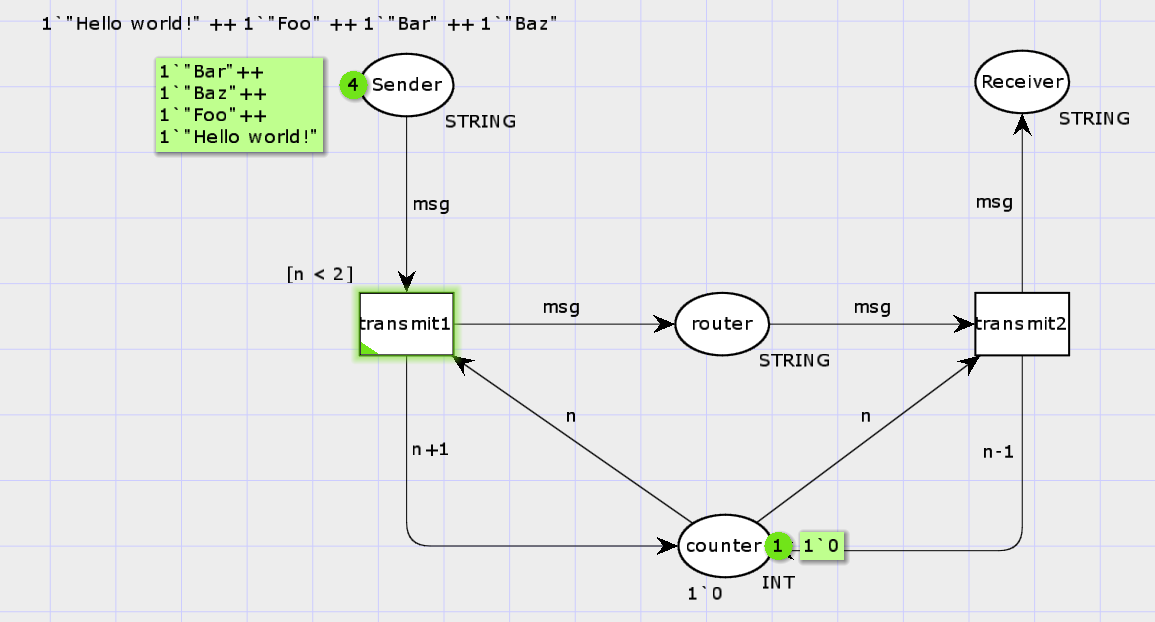
\includegraphics[width=11cm]{cpn_example.png}
\end{center}
\end{frame}

\subsection{CPN Tools}
\begin{frame}
\frametitle{CPN Tools}
\begin{myitemize}
  \item Tool for modeling and simulating Petri nets
  \item Support for exhaustive verification \& model checking
  \item Based on functional programming language ML
  \item Hierarchy support
  \item Open Source
  \item Active development
  \item Documentation and video tutorials available \url{http://cpntools.org/}
\end{myitemize}
\end{frame}

\subsection{Start of Mission Model}
\begin{frame}
\frametitle{Model of ``Start of Mission''}
\begin{itemize}
\item ``Start of Mission'' modeled according to spec
\item Model available on GitHub
\item Several issues identified (document in work)
\end{itemize}
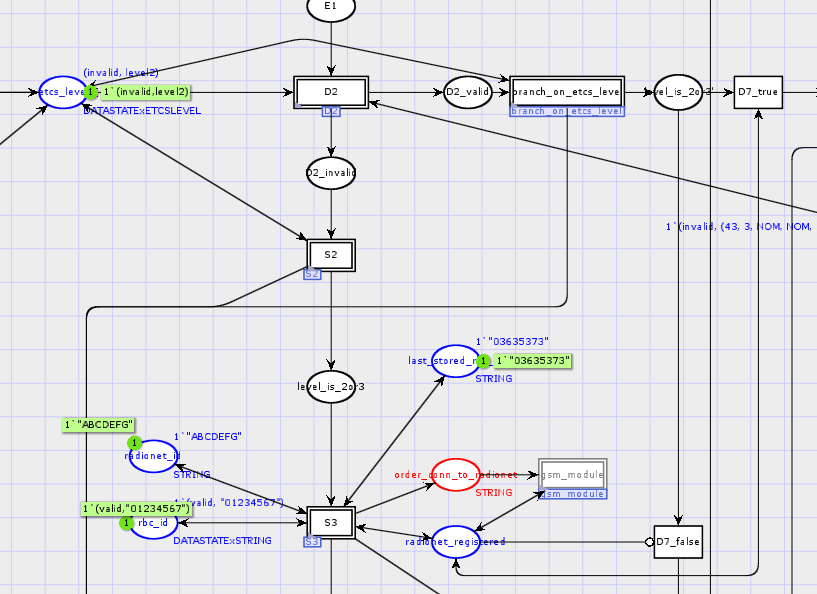
\includegraphics[width=8cm]{som_excerpt.png}
\end{frame}



\end{document}


